\documentclass[11pt]{article}
\usepackage[margin=0.9in]{geometry}
\usepackage{amsmath,amssymb,amsthm,booktabs,graphicx,hyperref,microtype,enumitem}
\hypersetup{colorlinks=true,linkcolor=blue,urlcolor=blue,citecolor=blue}
\newtheorem{proposition}{Proposition}
\newtheorem{definition}{Definition}
\newcommand{\R}{\mathbb R}
\newcommand{\C}{\mathbb C}
\newcommand{\tr}{\operatorname{tr}}
\newcommand{\rank}{\operatorname{rank}}
\title{Peeling Cascades and What They Leave Behind\\\large Channel Loss, Boundary Memory, and Elemental Inference}
\author{Jeromie N. Beasley\\\small Operator-first research program}
\date{Research draft 1 --- 7 September 2026}
\begin{document}
\maketitle
\begin{abstract}
A decrease in observed response does not uniquely identify the removal of a constituent. We formulate a peeling cascade as a sequence of declared interventions together with retained observables. For fixed real channel amplitudes with decreasing nonnegative weights, the response forms decrease in Loewner order and their kernels form an increasing filtration. Coordinate elimination has a different signature: exact Schur reduction preserves a boundary resolvent while placing hidden variables into frequency-dependent self-energy and time-dependent memory. A finite-dimensional moment certificate separates all-frequency transfer silence from an isolated cancellation, and examples show that the first nonzero memory moment can be delayed to the dimension-dependent bound. Two counterexamples delimit spectral interpretations: a two-sided boundary census can increase during positive-operator decrease, and zero normalized permutation entropy does not uniquely identify transposition defects. A reproducible Compound Eye implementation adds eight methods and executes 350 declared-model evaluations, including three expected rejections. These results establish an operational framework and falsification suite for elemental cascade inference; they do not establish an atomic removal law or fit experimental data.
\end{abstract}

\section{The question that a peel must answer}
An ``elemental peel'' can refer to electron emission, nuclear transformation, the suppression of an accessible transition, or the elimination of coordinates from a model. These operations need not agree. The present paper takes the channel-level question as its mathematical core and specifies what additional observations would justify an elemental interpretation.

We distinguish three levels of claim. An algebraic identity is conditional on a declared operator model. An inference identifies a model property from specified observations. A physical claim connects that property to a prepared species and a measured intervention. Passing an algebraic test does not supply this last connection. In particular, neither an atomic number nor a knot crossing number is inferred from an operator rank. We use $Z$ for proton number, $A_{\mathrm{nuc}}$ for nuclear mass number, $N_e$ for electron count, $c(K)$ for minimal knot crossing number, and $q$ for hidden-state dimension. The ambiguous historical label CN is not used.

\begin{definition}
A finite peeling experiment consists of operators $H_s$, declared interventions $\mathcal I_s$, preparation data, and measurement maps $\mathcal M_s$, indexed by a step $s$. A channel peel is the more restrictive family of positive response forms in Section 2. A coordinate peel is a nested sequence of retained subspaces with exact elimination of their complements. A physical peel requires an independently specified change in constituent content.
\end{definition}

A useful record therefore contains both what was changed and what was measured. A darkened detector can arise from a smaller weight, destructive interference, a rotated probe, shifted thresholds, altered preparation, or physical emission. The proposed instrument tests these alternatives separately, including cases in which the correct result is that the available readout is insufficient.

\section{Positive channel peeling and its exact limit}
Let $v_i\in\R^p$ be fixed channel vectors and let
\begin{equation}
G_s=\sum_{i=1}^{m}w_i^{(s)}v_i v_i^{\mathsf T},\qquad
0\leq w_i^{(s+1)}\leq w_i^{(s)}.
\label{eq:gram}
\end{equation}
The measured quadratic response to a real probe $e$ is $e^{\mathsf T}G_se$. The channel vectors, probe coordinates, and weight units must remain compatible across the comparison.

\begin{proposition}[Kernel filtration]
For the family in Eq.~\eqref{eq:gram}, $0\preceq G_{s+1}\preceq G_s$, and
\begin{equation}
\ker G_s=\bigcap_{i:w_i^{(s)}>0}v_i^\perp,
\qquad \ker G_s\subseteq\ker G_{s+1}.
\end{equation}
Consequently, rank cannot increase. Its decrease equals the decrease in the dimension of the span of active channel vectors. Changing strictly positive weights while preserving their support leaves the kernel unchanged.
\end{proposition}
\begin{proof}
For every $e$, $e^{\mathsf T}G_se=\sum_i w_i^{(s)}(v_i^{\mathsf T}e)^2$. Nonnegativity makes this sum zero exactly when every active amplitude vanishes. Subtracting consecutive forms proves Loewner order. The kernel formula then gives inclusion; rank follows from rank--nullity or the dimension of the active span.
\end{proof}

A removed channel need not lower rank. In the implemented example,
\begin{equation}
v_1=(1,0,0),\quad v_2=(0,1,0),\quad v_3=(1,1,0),\quad v_4=(0,0,1).
\end{equation}
Beginning with unit weights and removing $v_3,v_2,v_4,v_1$ gives ranks $3,3,2,1,0$. The first removal eliminates a redundant vector. Uniform attenuation to $10^{-12}$ keeps exact rank three. A numerical rank threshold can report a different answer; it must be recorded as a measurement or computational threshold, not silently promoted to exact rank.

The fixed-amplitude assumption is substantive. Electronic relaxation can change transition amplitudes after ionization. If the $v_i$ change, a comparison of weights alone does not establish Eq.~\eqref{eq:gram}. Signed or complex interference amplitudes also require a different model. A scalar rational response can vanish while every channel remains coupled: $1/(z-1)+1/(z-2)$ vanishes at $z=3/2$ but is not the zero transfer function. The instrument retains the earlier optical tune-out control for this reason.

\subsection{What a probe can identify}
For a real symmetric $p\times p$ form $G$, the $p(p+1)/2$ readings at $e_j$ and $e_j+e_k$ reconstruct it by polarization:
\begin{equation}
G_{jk}=\tfrac12\bigl[Q(e_j+e_k)-Q(e_j)-Q(e_k)\bigr],\quad j\ne k.
\end{equation}
This is noiseless form tomography, not constituent tomography. Many different channel factorizations yield the same $G$. Complex Hermitian forms require additional phase-sensitive probes. A single probe can lie in a kernel even when the form has large rank; comparing only that probe cannot certify a global peel.

\section{Coordinate peeling preserves a boundary through memory}
Partition a finite operator into retained and hidden coordinates,
\begin{equation}
H=\begin{pmatrix}A&B\\ C&D\end{pmatrix},\qquad
S(z)=zI-A-B(zI-D)^{-1}C.
\label{eq:schur}
\end{equation}
Here $H$ may be nonnormal; Hermiticity is not required for the algebra. If $zI-D$ and $zI-H$ are invertible, block inversion gives
\begin{equation}
\bigl[(zI-H)^{-1}\bigr]_{\mathrm{retained}}=S(z)^{-1}.
\label{eq:resolvent}
\end{equation}
The hidden sector survives as the self-energy $\Sigma(z)=B(zI-D)^{-1}C$. Bare deletion replaces $S(z)$ by $zI-A$ and normally changes the boundary response.

\begin{proposition}[Nested elimination]
For nested retained coordinate sets, successive Schur complements equal direct elimination to the final retained set wherever the required elimination blocks are invertible.
\end{proposition}
\begin{proof}
Solve the hidden block equations for an arbitrary forcing supported on the final retained coordinates. Solving all eliminated coordinates simultaneously or successively gives the same solution of the same invertible block system. Substitution into the retained equations therefore yields the same reduced pencil. Equivalently, block Gaussian elimination gives the Schur quotient identity.
\end{proof}

These are established reduction identities, closely related to Feshbach--Schur methods and Kron reduction \cite{feshbach,kron}. Their role here is diagnostic. A coordinate peel can preserve everything visible at the declared boundary even though the written state vector becomes shorter. This is not evidence that hidden physical constituents were destroyed. At poles, one must change the block or contour, or formulate an appropriate meromorphic statement; the numerical instrument blocks a singular pivot rather than inventing a finite inverse.

The corresponding time-domain statement makes the retained memory explicit. For $\dot x=Ax+By$, $\dot y=Cx+Dy$,
\begin{equation}
\dot x(t)=Ax(t)+\int_0^t B e^{(t-u)D}C x(u)\,du+B e^{tD}y(0).
\label{eq:memory}
\end{equation}
Variation of constants proves this identity directly. The final term records hidden initial preparation and cannot generally be dropped. For quantum unitary evolution the generator is $-iH/\hbar$, so the corresponding factors must be included. Our time-domain example is a declared linear model, not an atomic Hamiltonian simulation.

This provides a precise, limited sense in which memory can be ``built in'': an exactly eliminated sector leaves a convolution kernel and an initial-state forcing term. It does not establish a new fundamental memory field or a topological quantum field theory. The June 2026 preprint of Wang, Benner and Heiland explicitly develops the relation between partial observation, Mori--Zwanzig structure and variation of constants \cite{mz}. Our claim is an application to intervention discrimination with finite certificates, not priority for Eq.~\eqref{eq:memory}.

\section{A finite test for hidden transfer}
A dark response at one frequency does not establish that an eliminated sector is invisible. Finite dimension nevertheless provides a complete algebraic test.

\begin{proposition}[Finite transfer-silence certificate]
Let $D\in\C^{q\times q}$ with $q\geq1$, and let $B,C$ be compatible matrices. The following statements are equivalent:
\begin{enumerate}[nosep]
\item $B(zI-D)^{-1}C$ is identically zero as a rational matrix;
\item $BD^jC=0$ for $j=0,\ldots,q-1$;
\item $Be^{tD}C=0$ for every $t$.
\end{enumerate}
These statements concern the input-to-output hidden transfer. Absence of hidden-initial-state forcing additionally requires $BD^jy(0)=0$ for $j=0,\ldots,q-1$.
\end{proposition}
\begin{proof}
For sufficiently large $|z|$, the resolvent has the convergent expansion $\sum_{j\geq0}D^jz^{-j-1}$. Rational transfer silence thus implies all its Laurent coefficients vanish. By Cayley--Hamilton, vanishing of the first $q$ moments implies vanishing of every subsequent moment. The exponential power series then gives statement 3, and its derivatives at zero give the converse. Applying the same argument to the vector $y(0)$ proves the forcing criterion.
\end{proof}

The bound cannot be shortened uniformly. Let $D=N_q$ have ones on the first superdiagonal and zeros elsewhere, $B=e_1^{\mathsf T}$, and $C=e_q$. Then
\begin{equation}
BD^jC=0\ (j<q-1),\quad BD^{q-1}C=1,\qquad
\Sigma(z)=z^{-q}.
\end{equation}
Thus $q-1$ leading zero moments can precede a nonzero response. The implemented exact examples use $q=1,\ldots,5$; the displayed argument proves the arbitrary finite-dimensional statement. If stability is required, replacing $D$ with $-I+N_q$ preserves the delayed first nonzero moment and gives $(z+1)^{-q}$.

The suite also reports the rank of the finite block Hankel matrix $[BD^{j+k}C]_{j,k=0}^{q-1}$. This is an exact algebraic diagnostic of the example's transfer realization. It is not a robust order estimator for noisy measurements. A fitted finite-dimensional model needs an independently justified order bound before its first $q$ moments can be called a complete physical certificate. Approximate zeros require error bounds; this paper's exact certificate does not provide them.

\section{Two spectral traps that matter for the cascade}
\subsection{A boundary census need not decrease}
The source manuscript \emph{Matter at a Scale}, version 5, uses compressed projectors and a two-sided spectral window. For a positive contraction $C$ define
\begin{equation}
N_\epsilon(C)=\#\{\lambda\in\operatorname{spec}(C):\epsilon\leq\lambda\leq1-\epsilon\},\quad 0<\epsilon<1/2.
\end{equation}
This is not rank. Consider
\begin{equation}
C_0=\operatorname{diag}(0.99,0.5,0.01),\qquad
C_1=\operatorname{diag}(0.8,0.4,0).
\end{equation}
Then $0\preceq C_1\preceq C_0$, trace decreases from $1.5$ to $1.2$, and rank decreases from three to two. Nevertheless $N_{0.1}$ increases from one to two. These contractions are legitimate projector compressions: for each,
\begin{equation}
P(C)=\begin{pmatrix}C&\sqrt{C(I-C)}\\\sqrt{C(I-C)}&I-C\end{pmatrix}
\end{equation}
is an orthogonal projector. This does not assert that the two dilated projectors themselves form a Loewner-decreasing family. It establishes that compression alone does not exclude the counterexample.

Consequently, a boundary census can be retained as a scale-dependent observable, but cannot be identified with removed electrons or a monotonically decreasing channel number. Likewise, affine covariance requires consistent energy references: if $H'=aH+bI$, $z'=az+b$, $a>0$, then $(z'I-H')^{-1}=a^{-1}(zI-H)^{-1}$. A fixed external chemical potential or detector threshold is additional data and need not select the same cluster after this transformation.

\subsection{Zero normalized entropy has two cycle classes}
The new permutation source provides another useful stress test. For a permutation matrix $P$, write
\begin{equation}
G=\tfrac12(P-I)^{\mathsf T}(P-I)=I-\tfrac12(P+P^{\mathsf T}).
\end{equation}
An $\ell$-cycle contributes eigenvalues $2\sin^2(\pi j/\ell)$, $j=0,\ldots,\ell-1$. For a nonidentity permutation, normalize by $\lambda_{\max}$ and set $\mathcal H=\sum_j h(\lambda_j/\lambda_{\max})$, where $h(u)=-u\log u-(1-u)\log(1-u)$ and $h(0)=h(1)=0$.

\begin{proposition}[Corrected zero-entropy classification]
$\mathcal H=0$ exactly when all nontrivial cycles have length two, or all nontrivial cycles have length three. Arbitrary fixed points are allowed in either case.
\end{proposition}
\begin{proof}
Binary entropy is positive strictly inside $(0,1)$, so zero entropy means that all positive eigenvalues of $G$ are equal. A two-cycle contributes only the positive value $2$; a three-cycle contributes only $3/2$, twice. Mixing these lengths gives two distinct positive values. Every cycle of length at least four already has unequal positive eigenvalues, as seen by comparing $j=1$ and $j=\lfloor\ell/2\rfloor$. These observations prove both directions.
\end{proof}

The earlier transposition-only interpretation is therefore too restrictive. In the same ambient dimension four, cycle types $(2,2)$ and $(3,1)$ both have normalized spectrum $(0,0,1,1)$, but their moved-point counts are four and three, and their spectral maxima are $2$ and $3/2$. Thus even the entire normalized spectrum does not distinguish these examples. The instrument retains unnormalized scale, moved support, ambient dimension and threshold convention. Its exhaustive partition controls through dimension twelve agree with the proved classification. Permutation cycles here are not knot crossing numbers; the result supplies no elemental knot assignment.

\section{Compound Eye implementation and results}
The focused extension adds eight versioned methods to the existing instrument. All 150 pre-existing eye specifications are checked against stored hashes and preserved. The resulting registry has 158 versions; this does not mean that every registered historical proposal is executable or relevant to this paper.

\begin{center}\small
\begin{tabular}{p{0.25\linewidth}p{0.64\linewidth}}
\toprule
New method & Tested question\\\midrule
Positive peel & Does exact fixed-channel removal obey kernel inclusion?\\
Schur cascade & Does nested elimination preserve the same boundary response?\\
Memory certificate & Do the first $q$ exact transfer moments certify silence?\\
Time memory & Does variation of constants retain history and preparation?\\
Cycle profile & What is lost through spectral normalization?\\
Window census & Can a two-sided count increase under positive decrease?\\
Tomography & Can complete real quadratic probes reconstruct the form?\\
Affine scale & Was the energy reference transformed consistently?\\\bottomrule
\end{tabular}
\end{center}

The deterministic run executes 350 eye evaluations: 347 return successfully and three are deliberately blocked. The blocked cases are increasing channel weights, a singular Schur pivot, and a corrupted earlier Fox-calculus control. There are 259 nonidentity permutation partition controls in dimensions two through twelve. Additional checks outside the eye dispatcher establish an exact rational nested Schur identity and verify the projector dilations numerically. An evaluation count is not a count of independent discoveries or experimental validations.

The Schur tests cover all six orders for eliminating three interior coordinates of a seeded five-dimensional symmetric model at three complex energies, and a twelve-site chain at 25 energies with three nested reductions. Assertions require boundary residuals below $10^{-10}$ for the chain. The comparison with bare deletion demonstrates the cost of dropping self-energy. Time-memory tests use two initial preparations and five times; they evaluate the convolution along the full reference trajectory and check Eq.~\eqref{eq:memory} to $10^{-10}$. They do not constitute an independently integrated reduced-memory solver.

Selected existing optical, pairing, nonnormality, recycling, modular-translation, Cheshire-cat and knot admission controls also run. These are controls on interpretation. They are not evidence that every one of those physical mechanisms occurs in an elemental cascade. In particular, a nonunitary representation is not silently admitted to a self-adjoint APS construction. No APS or knot-volume theorem is required for Propositions 1--4.

\begin{figure}[htbp]
\centering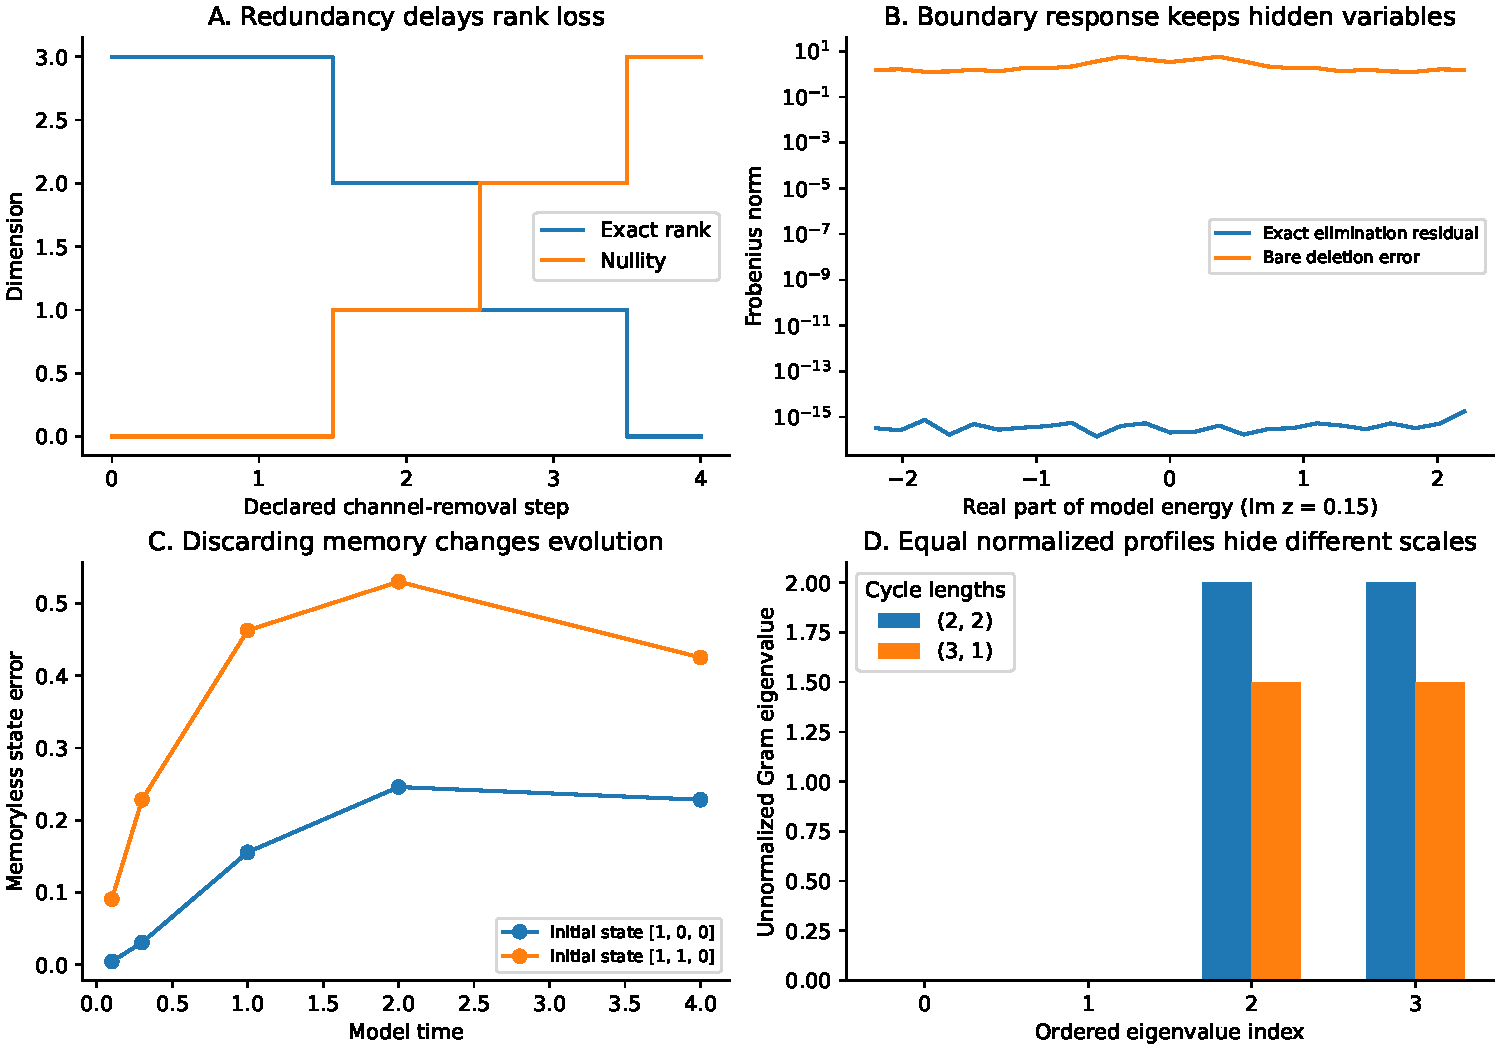
\includegraphics[width=\linewidth]{cascade_controls.pdf}
\caption{Declared-model controls. (A) Redundant channel removal precedes rank loss. (B) Exact boundary reduction agrees with the full resolvent while bare deletion changes it. (C) Dropping hidden memory changes the retained evolution for both preparations. (D) Two permutation types have equal normalized spectra but distinct unnormalized scales. All panels are synthetic calculations.}
\end{figure}

\subsection{Formal proof coverage}
The package retains the earlier Lean module \texttt{OpticalMetric.lean}, its project configuration and archived verification evidence. The recorded build, axiom audit and independent checker cover 16 declarations, including four positive-weight/peeling results. Its SHA-256 is verified against the archived report. This turn did not recompile Lean: a compiler was unavailable locally. The new Schur, finite-memory and permutation statements in this manuscript have written proofs and computational controls; they are not claimed to have new Lean certificates. An archived successful build and a fresh numerical run are reported separately.

\section{Position relative to the current landscape}
The strongest publication position is a methods paper about what a cascade observation identifies, supported by reproducible failure controls. It is not a claim to replace experimental ionization theory or outperform unmeasured competitors.

\begin{itemize}[leftmargin=*]
\item Feshbach--Schur theory and electrical Kron reduction already provide exact elimination tools \cite{feshbach,kron}. Here they distinguish coordinate removal from changed boundary physics.
\item The 2026 Mori--Zwanzig preprint gives explicit linear partial-observation memory formulas \cite{mz}. Our finite silence test and delayed-moment controls specify what a zero readout can and cannot establish within a bounded model class.
\item Simmermacher and collaborators image changes in electron-pair density during molecular Auger--Meitner decay \cite{auger}. This is a direct experimental target for separating actual electron loss from redistribution in an observed response. We have not reanalysed its raw measurements.
\item Koll and collaborators study electronic coherence and ion--photoelectron entanglement in attosecond molecular photoionization \cite{koll}. This motivates retaining preparation and coherence information alongside any constituent-count record. It does not identify their coherence observable with our Gram rank.
\end{itemize}

The source comparison was checked on 7 September 2026. This is a targeted comparison, not an exhaustive novelty search. The elementary matrix identities and classical reduction methods are attributed as such. The proposed contribution is their combined use as a falsifiable cascade classification, with explicit counterexamples and a reusable implementation. Establishing methodological superiority still requires a common data task, baselines, uncertainty estimates and held-out evaluation.

\section{From the operator result to an elemental test}
The next physical test should specify a single system and intervention, rather than fit a universal element--knot table. A workable candidate is a prepared atom or molecule undergoing controlled photoionization followed by a resolved decay cascade. The minimum record is
\begin{equation}
\mathcal D=(Z,A_{\mathrm{nuc}},N_e,\text{preparation},\text{pulse},\text{outgoing channels},\text{probe},\text{calibration}).
\end{equation}
For molecules, constituent species and charge states replace a single-species shorthand. Detector events and calibration records must be distinguished from derived spectra and model reconstructions. No such raw experimental dataset is fitted in this release.

A useful first comparison has three models: a bare-deletion model, an exact or controlled memory reduction, and a response-only attenuation model. They must predict the same held-out observable with the same preparation information. Training and validation should be separated by acquisition blocks or preparations rather than correlated adjacent samples. A numerical eigenvalue cutoff should be swept against measured uncertainty. A physical emission claim should use independently resolved outgoing channels or charge-state evidence; a declining optical signal alone is insufficient.

The fixed-channel theorem has a clear failure condition: after verifying comparable probes and positive weights, a measured increase of the response form beyond uncertainty rejects that particular fixed-channel peel model. It does not reject all possible cascades. Conversely, agreement with monotone forms does not uniquely identify the channels or certify electron removal. A successful memory model must predict withheld time or frequency responses rather than merely reproduce the trajectory used to calculate its convolution.

Nuclear removal is a separate experiment with nuclear species and reaction bookkeeping. Nothing in the present finite-dimensional proof predicts the mass-five or mass-eight bottlenecks. Nor does a permutation spectrum establish a knot invariant, a conductivity law, or an emergent gravitational metric. Those possible bridges require specified operators, observables and independent tests.

\section{Conclusion}
A peeling cascade becomes mathematically informative when its intervention is explicit. Positive fixed-channel removal enlarges null spaces; exact coordinate elimination preserves a declared boundary by retaining self-energy and memory; a measured zero can be only a cancellation or a probe restriction. Spectral normalization and windowing can erase distinctions essential to interpretation. The resulting paper and instrument provide an operational starting point for an elemental experiment, with exact algebraic limits and reproducible counterexamples. The unresolved step is empirical: linking a specified physical removal process to an identifiable operator family using raw calibrated observations.

\section*{Reproducibility and provenance}
The accompanying archive contains the full instrument snapshot, eight new methods, the deterministic runner, its 350 input/output records, figure source, manuscript source, an Atlas-to-claim map, source hashes and the archived Lean evidence. Run \texttt{python run\_cascade.py} from the extracted package after installing the declared dependencies; \texttt{python make\_figures.py} rebuilds the figure. The wrapper resolves paths relative to itself. No GitHub checkout is needed for these calculations. Lean dependencies are separately configured and must be obtained for a new Lean build. AI assistance was used for synthesis, programming and checking; its outputs are not treated as independent experimental evidence. The author should review all claims and journal-specific disclosure requirements before submission.

\begin{thebibliography}{9}
\bibitem{kron} F. D\"orfler and F. Bullo, \emph{Kron Reduction of Graphs with Applications to Electrical Networks}, IEEE Transactions on Circuits and Systems I (2013). \url{https://arxiv.org/abs/1102.2950}.
\bibitem{feshbach} M. Griesemer and D. Hasler, \emph{On the Smooth Feshbach--Schur Map} (2007). \url{https://arxiv.org/abs/0704.3244}.
\bibitem{mz} F. Wang, P. Benner and J. Heiland, \emph{Partial Observation of Linear Systems with the Mori--Zwanzig Formalism}, arXiv:2606.23341v1 (22 June 2026), preprint. \url{https://arxiv.org/abs/2606.23341}.
\bibitem{auger} M. Simmermacher et al., \emph{Real-space imaging of the electron-pair density hole in molecular Auger--Meitner decay}, Nature Physics (2026). \url{https://doi.org/10.1038/s41567-026-03363-8}.
\bibitem{koll} L.-M. Koll et al., \emph{Entanglement and electronic coherence in attosecond molecular photoionization}, Nature (2026). \url{https://doi.org/10.1038/s41586-026-10230-2}.
\end{thebibliography}
\end{document}
